\documentclass[xcolor=table, 10pt, aspectratio=43]{beamer}

%\usepackage{arev}
\usepackage{amsmath,amssymb,amscd}
\usepackage{dsfont}
\usepackage{mathrsfs}
\usepackage{yfonts}
\usepackage{bm}
\usepackage{graphicx}
\usepackage{tabularx}
\usepackage{animate}
\usepackage{pifont}
%\usepackage{ifthen}

%\usepackage{xeCJK}
%\usepackage{fontspec}
%\newfontfamily\cjkfont{PingFang SC}
%\setCJKmainfont{PingFang SC}
\newcolumntype{x}{>{\centering\arraybackslash}X}
\renewcommand{\arraystretch}{1.5}

\usepackage{tikz}
	\usetikzlibrary{calc}
	\usetikzlibrary{arrows,shapes, positioning, matrix}
	\usetikzlibrary{decorations.markings}
	\tikzstyle arrowstyle=[scale=1]
	\tikzstyle directed=[postaction={decorate,decoration={markings,
 	   mark=at position .15 with {\arrow[arrowstyle]{stealth}}}}]
\tikzstyle string=[thick,postaction={decorate,decoration={markings,
    mark=at position .55 with {\arrow[arrowstyle]{stealth}}}}]
\tikzstyle dual_string=[dashed,postaction={decorate,decoration={markings,
    mark=at position .55 with {\arrow[arrowstyle]{stealth}}}}]

\tikzstyle dw=[thick,postaction={decorate,decoration={markings,
    mark=at position 1 with {\arrow[arrowstyle]{stealth}}}}]
\tikzstyle group=[mbg]

\usepackage{pgffor}
\newcommand{\mb}[1]{\mathbf{#1}}
\renewcommand{\cal}[1]{\mathcal{#1}}

\newcommand{\ag}[2]{#1_\mb{#2}}
\newcommand{\cohosub}[1]{\scalebox{0.72}{\textswab{#1}}}
\newcommand{\cohosubsub}[1]{\scalebox{0.6}{\textswab{#1}}}
\newcommand{\coho}[1]{\textswab{#1}}


\mode<presentation>
{
  %\usetheme{Warsaw}
  % or ...
  %\useoutertheme{rectangle}
  \setbeamertemplate{frametitle}[default][center]
  \defbeamertemplate{itemize item}{flat}{\begin{pgfpicture}{-1ex}{0ex}{1ex}{2ex}
      \pgfpathcircle{\pgfpoint{0pt}{.6ex}}{0.6ex}
      \pgfusepath{fill}
    \end{pgfpicture}%
  }
  \defbeamertemplate{itemize subitem}{flat}{\footnotesize\raise0.5pt\hbox{\textbullet}}
  \defbeamertemplate{itemize subsubitem}{flat}{\footnotesize\raise0.5pt\hbox{\textbullet}}

  %\useinnertheme{circles}
  \setbeamertemplate{items}[flat]
  \setbeamertemplate{sections/subsections in toc}[circle]
  \setbeamertemplate{blocks}[rounded]
  \setbeamertemplate{title page}[default][colsep=-4bp,rounded=true]
  \setbeamertemplate{part page}[default][colsep=-4bp,rounded=true]
  \setbeamercovered{transparent}
  %\usecolortheme{spruce}
  %\definecolor{THU}{RGB}{116,61,130}
  \definecolor{mbg}{RGB}{0,0,160}
  \setbeamercolor*{palette primary}{fg=white,bg=mbg}
  \setbeamercolor*{titlelike}{parent=palette primary}
  \setbeamercolor*{structure}{fg=mbg}
  \setbeamercolor{frametitle}{fg=white,bg=mbg}
  % or whatever (possibly just delete it)
  \setbeamercolor{block title}{bg=mbg,fg=white}
  \setbeamercolor{block body}{bg=mbg!15}


  \addtobeamertemplate{navigation symbols}{}{ \hspace{1em}%
    \usebeamerfont{footline}%
    \insertframenumber / \inserttotalframenumber }
}


%\usepackage[english]{babel}
% or whatever

%\usepackage[latin1]{inputenc}
% or whatever

%\usepackage{times}
%\usepackage[T1]{fontenc}
% Or whatever. Note that the encoding and the font should match. If T1
% does not look nice, try deleting the line with the fontenc.

\title[EQMC] % (optional, use only with long paper titles)
{Metals' awkward cousin is found}

\author[Y Qi] % (optional, use only with lots of authors)
{Yang~Qi}
% - Give the names in the same order as the appear in the paper.
% - Use the \inst{?} command only if the authors have different
%   affiliation.

\institute[Fudan] % (optional, but mostly needed)
{
Department of Physics, Fudan University.
}
% - Use the \inst command only if there are several affiliations.
% - Keep it simple, no one is interested in your street address.

%\date{2016 Annual Meeting of Fudan CFTPP} % (optional, should be abbreviation of conference name)
%{Fudan University, Oct 13 2015}
\date{SUSTech, May 17th 2019.}
% - Either use conference name or its abbreviation.
% - Not really informative to the audience, more for people (including
%   yourself) who are reading the slides online

\subject{Theoretical Physics}
% This is only inserted into the PDF information catalog. Can be left
% out.



% If you have a file called "university-logo-filename.xxx", where xxx
% is a graphic format that can be processed by latex or pdflatex,
% resp., then you can add a logo as follows:

\pgfdeclareimage[height=1cm]{university-logo}{../resources/fudan}
\logo{\pgfuseimage{university-logo}}



% Delete this, if you do not want the table of contents to pop up at
% the beginning of each subsection:
\AtBeginSection[]
{
  \begin{frame}<beamer>{Outline}
			\tableofcontents[currentsection,currentsubsection]
  \end{frame}
}
%\AtBeginSubsection[]
%{
 % \begin{frame}<beamer>{Outline}
  %  \tableofcontents[currentsection,currentsubsection]
  %\end{frame}
%}


\begin{document}

\begin{frame}
  \titlepage
\end{frame}

\begin{frame}{Collaborators}
\begin{itemize}
\item Chuang Chen, Institute of Physics, CAS.
\item Xiao Yan Xu, Hong Kong University of Science and Technology.
\item Zi Yang Meng, Hong Kong University.
\begin{center}
  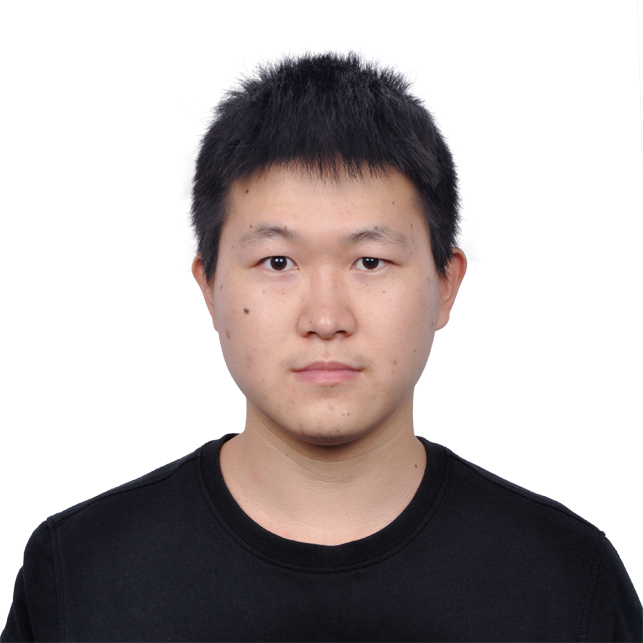
\includegraphics[height=2cm]{../people/chuangchen}
  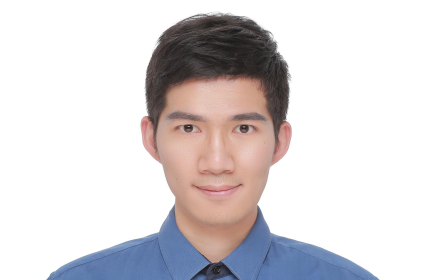
\includegraphics[height=2cm]{../people/xiaoyanxu}
  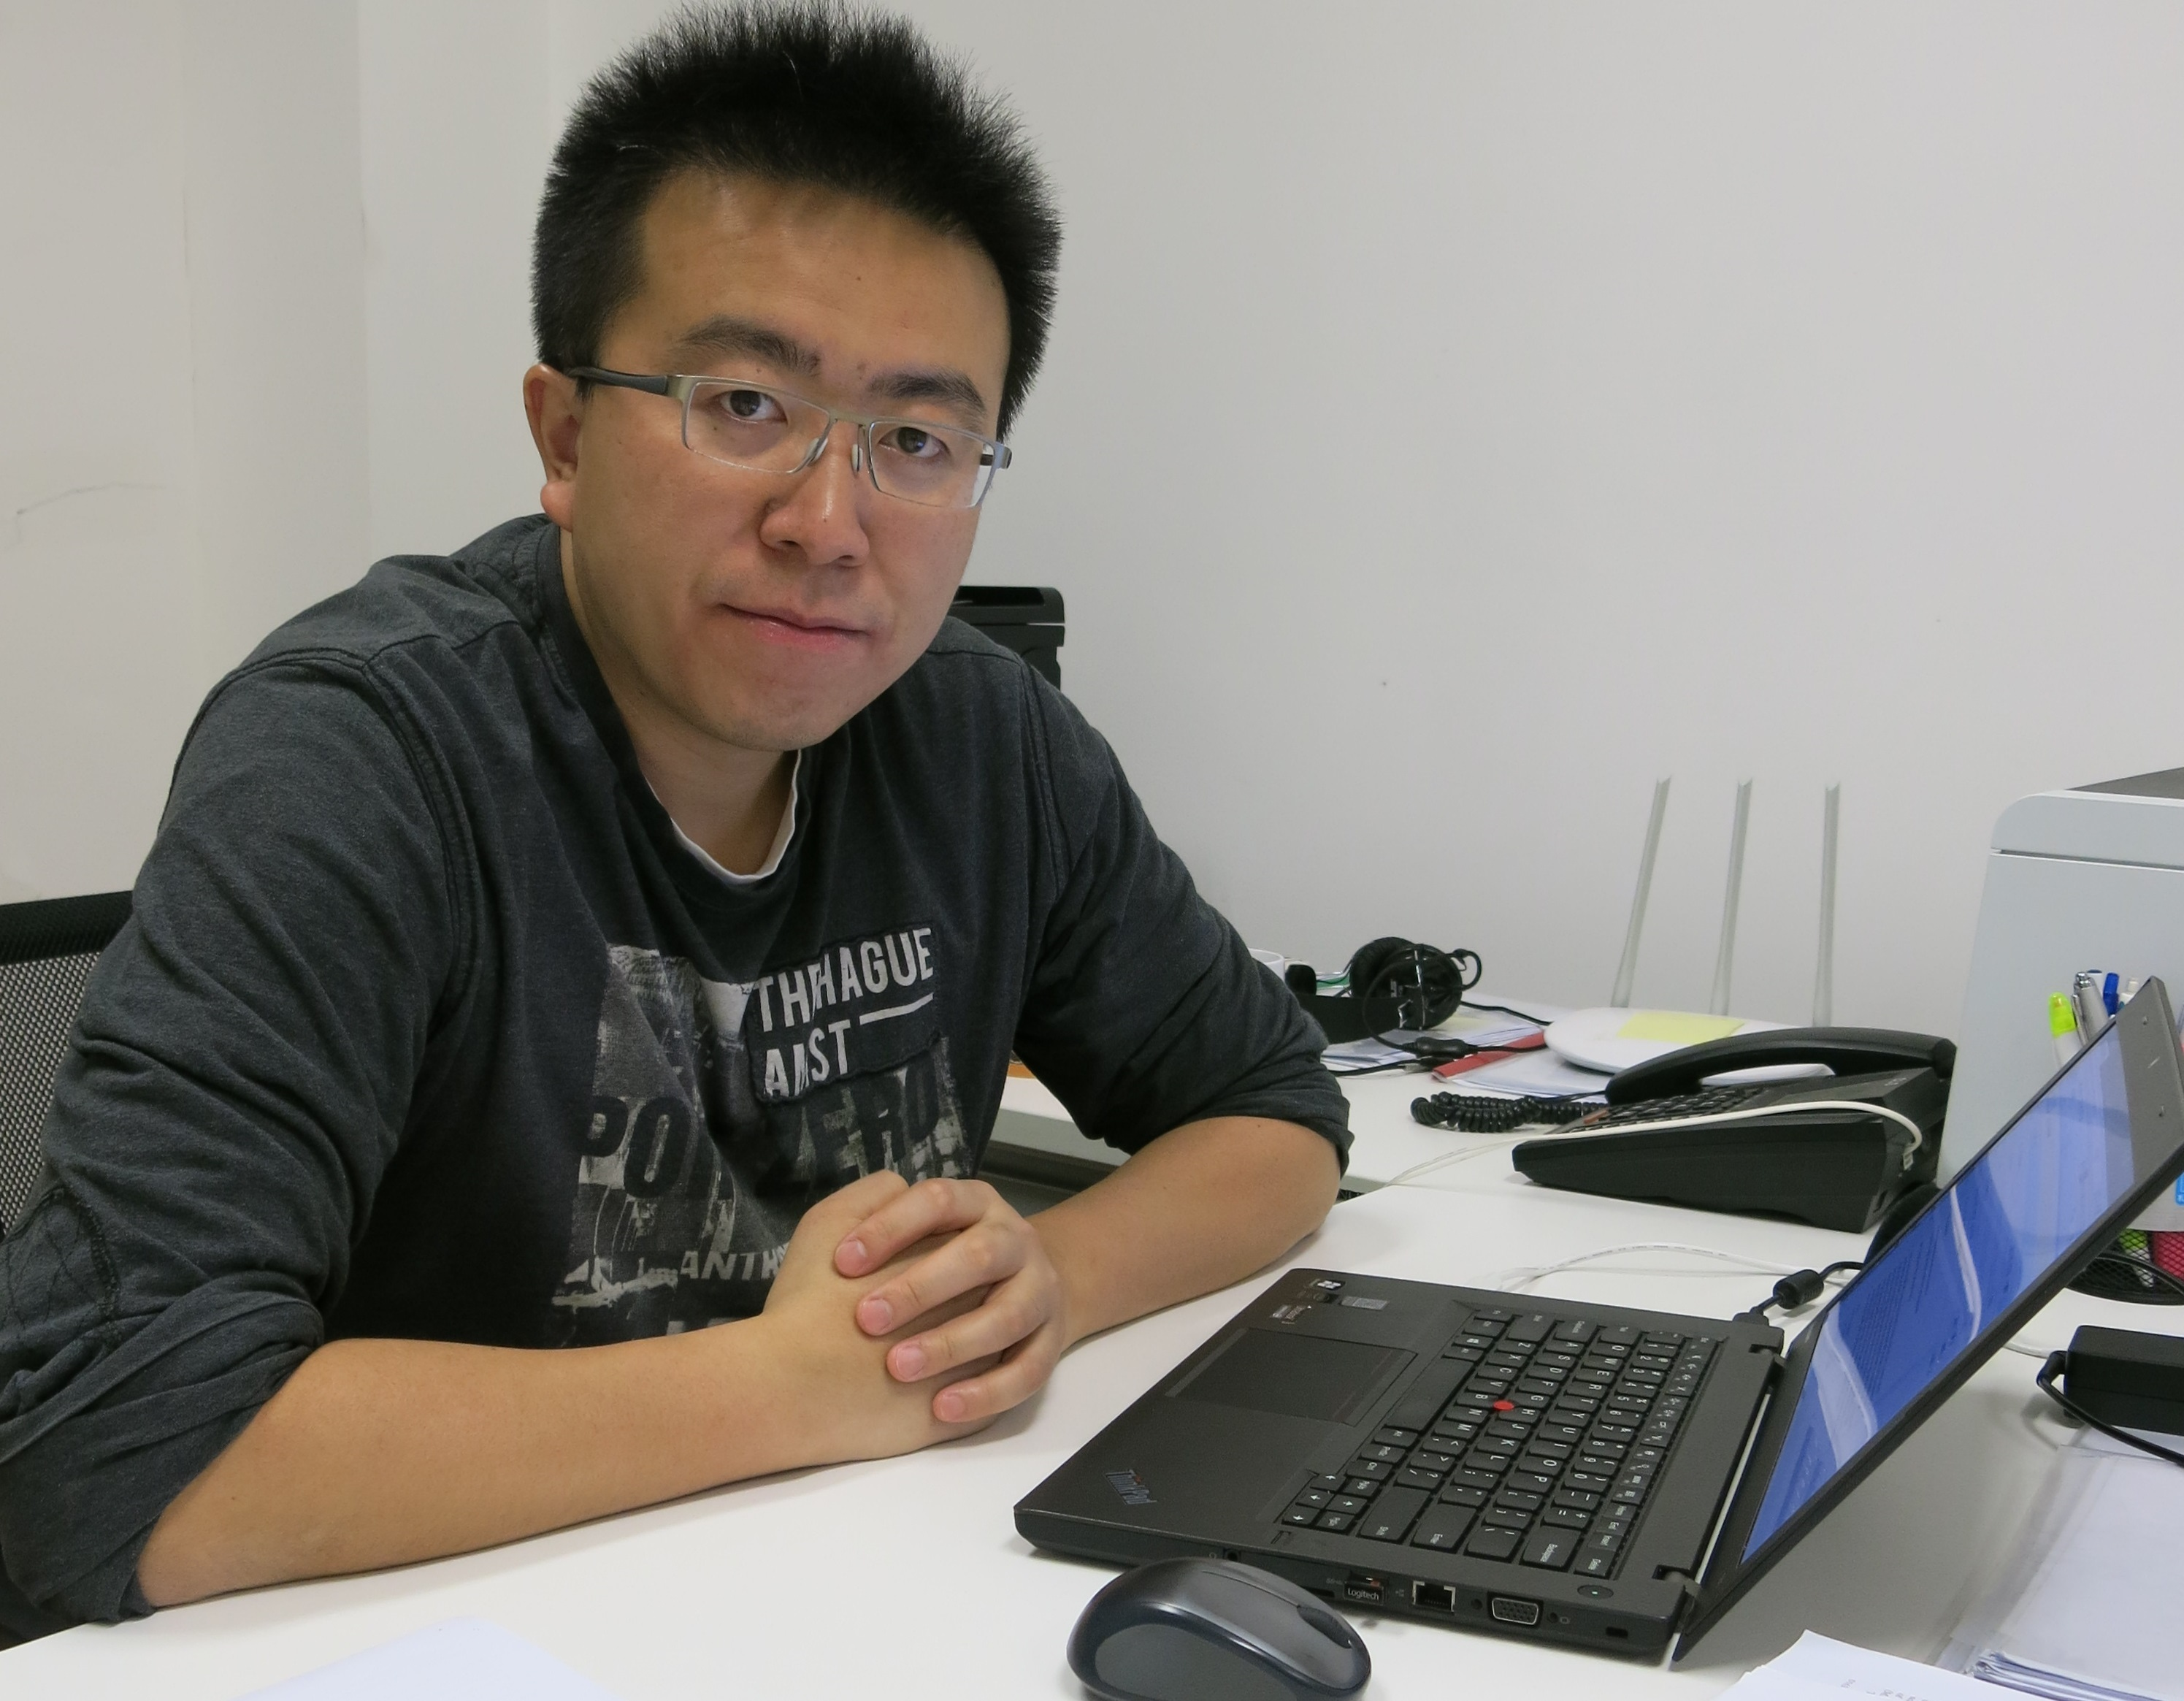
\includegraphics[height=2cm]{../people/ziyangmeng}
\end{center}
\end{itemize}
\begin{center}
  \small arXiv:1904.12872
\end{center}
\end{frame}

\begin{frame}{Outline}
	%\begin{columns}
	%\column{.7\textwidth}
		\tableofcontents
  %\end{columns}
  % You might wish to add the option [pausesections]
\end{frame}

\section{Introduction}

\begin{frame}
  \frametitle{Metal: Fermi surface}
\begin{itemize}
  \item Landau Fermi-Liquid Theory: a Fermi surface of quasiparticles.\\
  Noninteracting FS $\rightarrow$ Interacting FS.
  \item Volumn of the FS is conserved: Luttinger Thm.
\end{itemize}
\begin{center}
	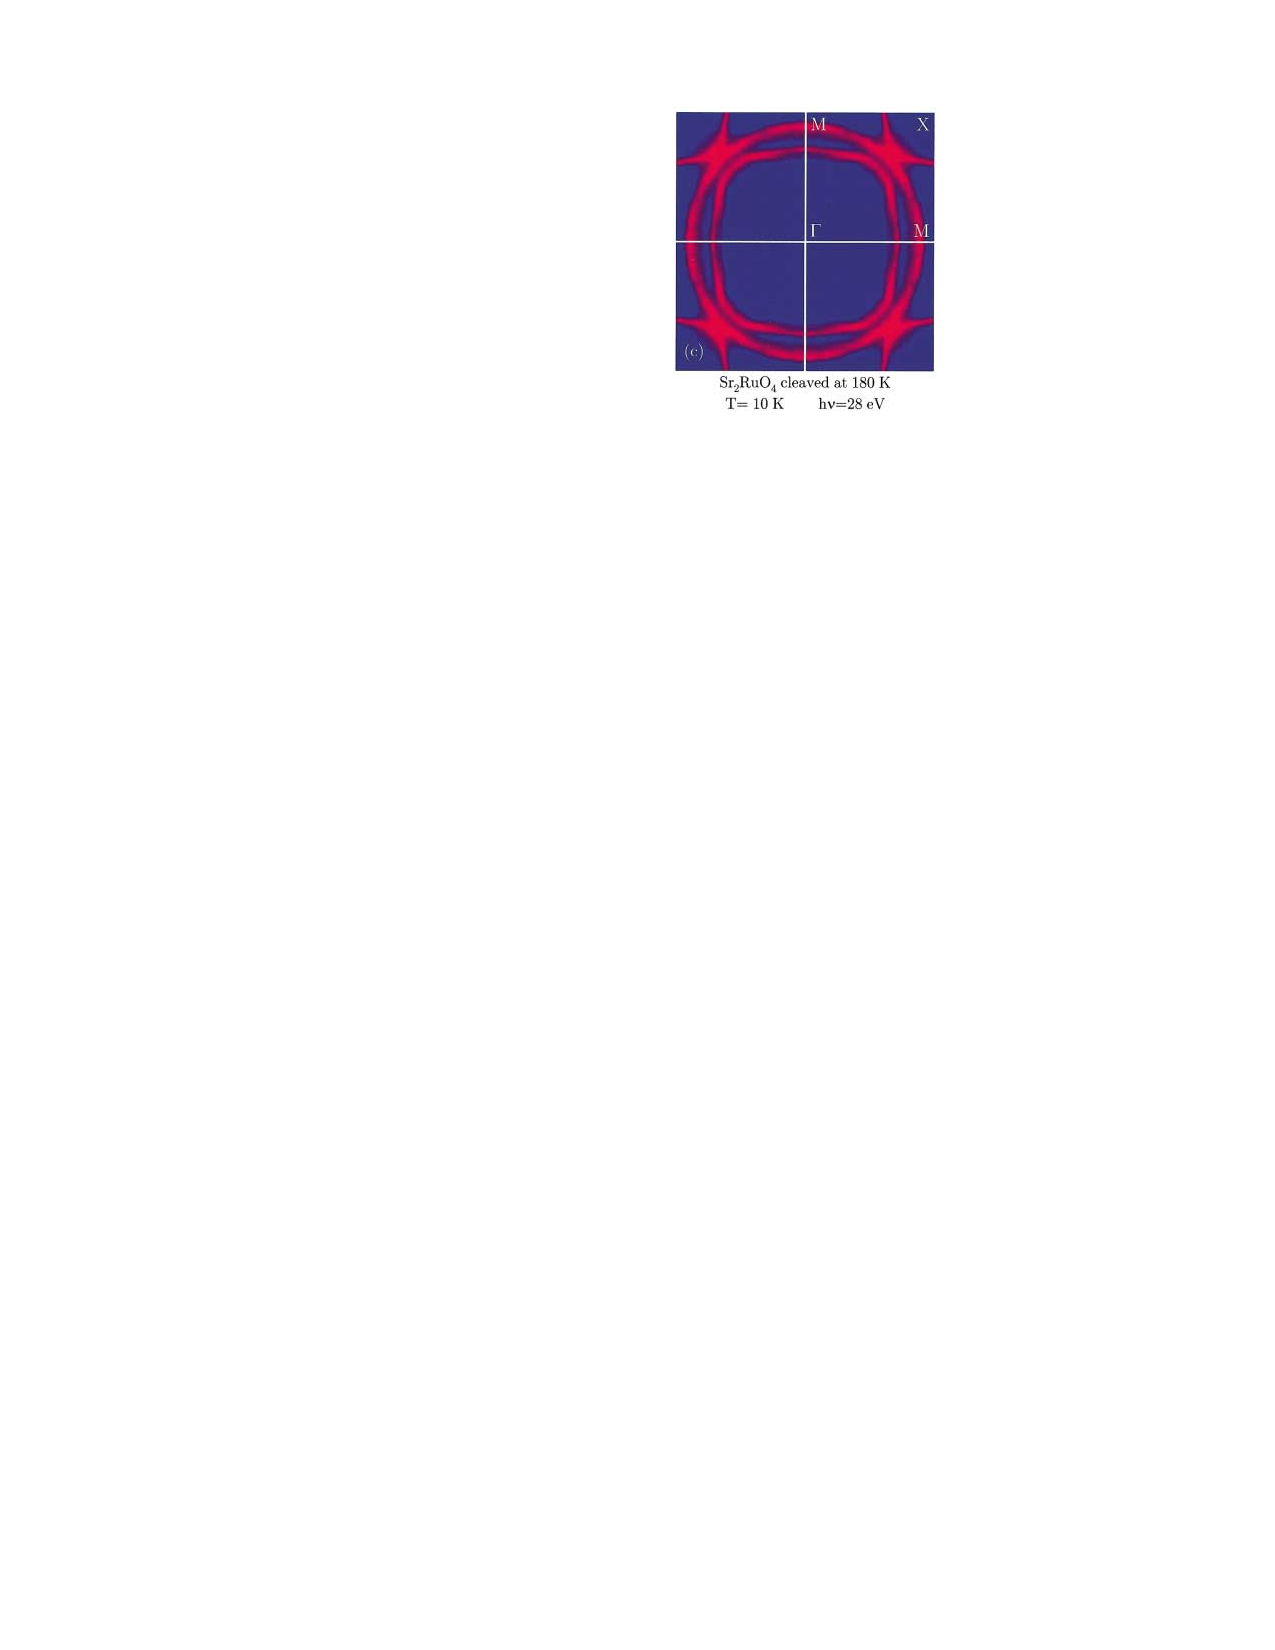
\includegraphics{../resources/SrRuO_FS}

	{\small A. Damascelli et al, PRL \textbf{85} 5194 (2000).}
\end{center}
\end{frame}

\begin{frame}
  \frametitle{Hiding an FS with Fractionalization}
  \begin{itemize}
    \item Spin-charge separation: $c_{i\alpha} = f_{i\alpha} h_i^\dagger$.
		\item $h$ forms a Mott insulator.
		\item No $c$-FS: no spectral weights.
		\item Generalized Luttinger Thm:
		$\nu_e = A_c + A_f$.
		\item Orthogonal metal: $\left<c^\dagger f\right>\rightarrow 0$.
  \end{itemize}
	\begin{center}
		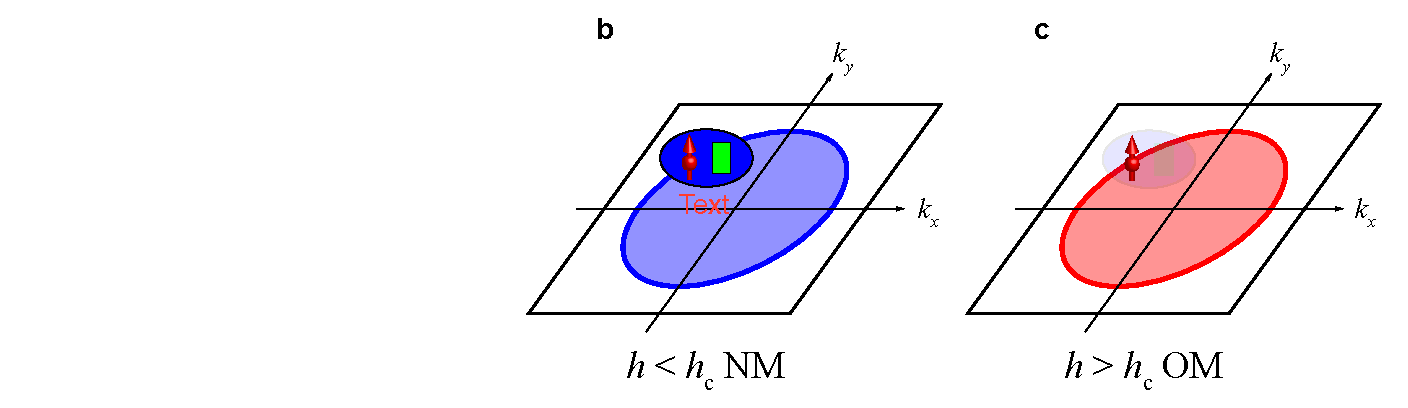
\includegraphics[width=.8\textwidth]{hide_fs}
	\end{center}
\end{frame}

\begin{frame}
	\frametitle{Questions to address}
	\begin{itemize}
		\item[\ding{51}] Realizing OM in a Monte Carlo simulation.
		\item[\ding{51}] Phase transition b/w NM/OM?
		\item[\ding{55}] Which realistic model realizes an OM?
		\item[\ding{55}] Which material realizes an OM?
	\end{itemize}

\end{frame}

\begin{frame}
\frametitle{Designer Hamiltonians}
\begin{columns}
	\column{.6\textwidth}
	\begin{center}
		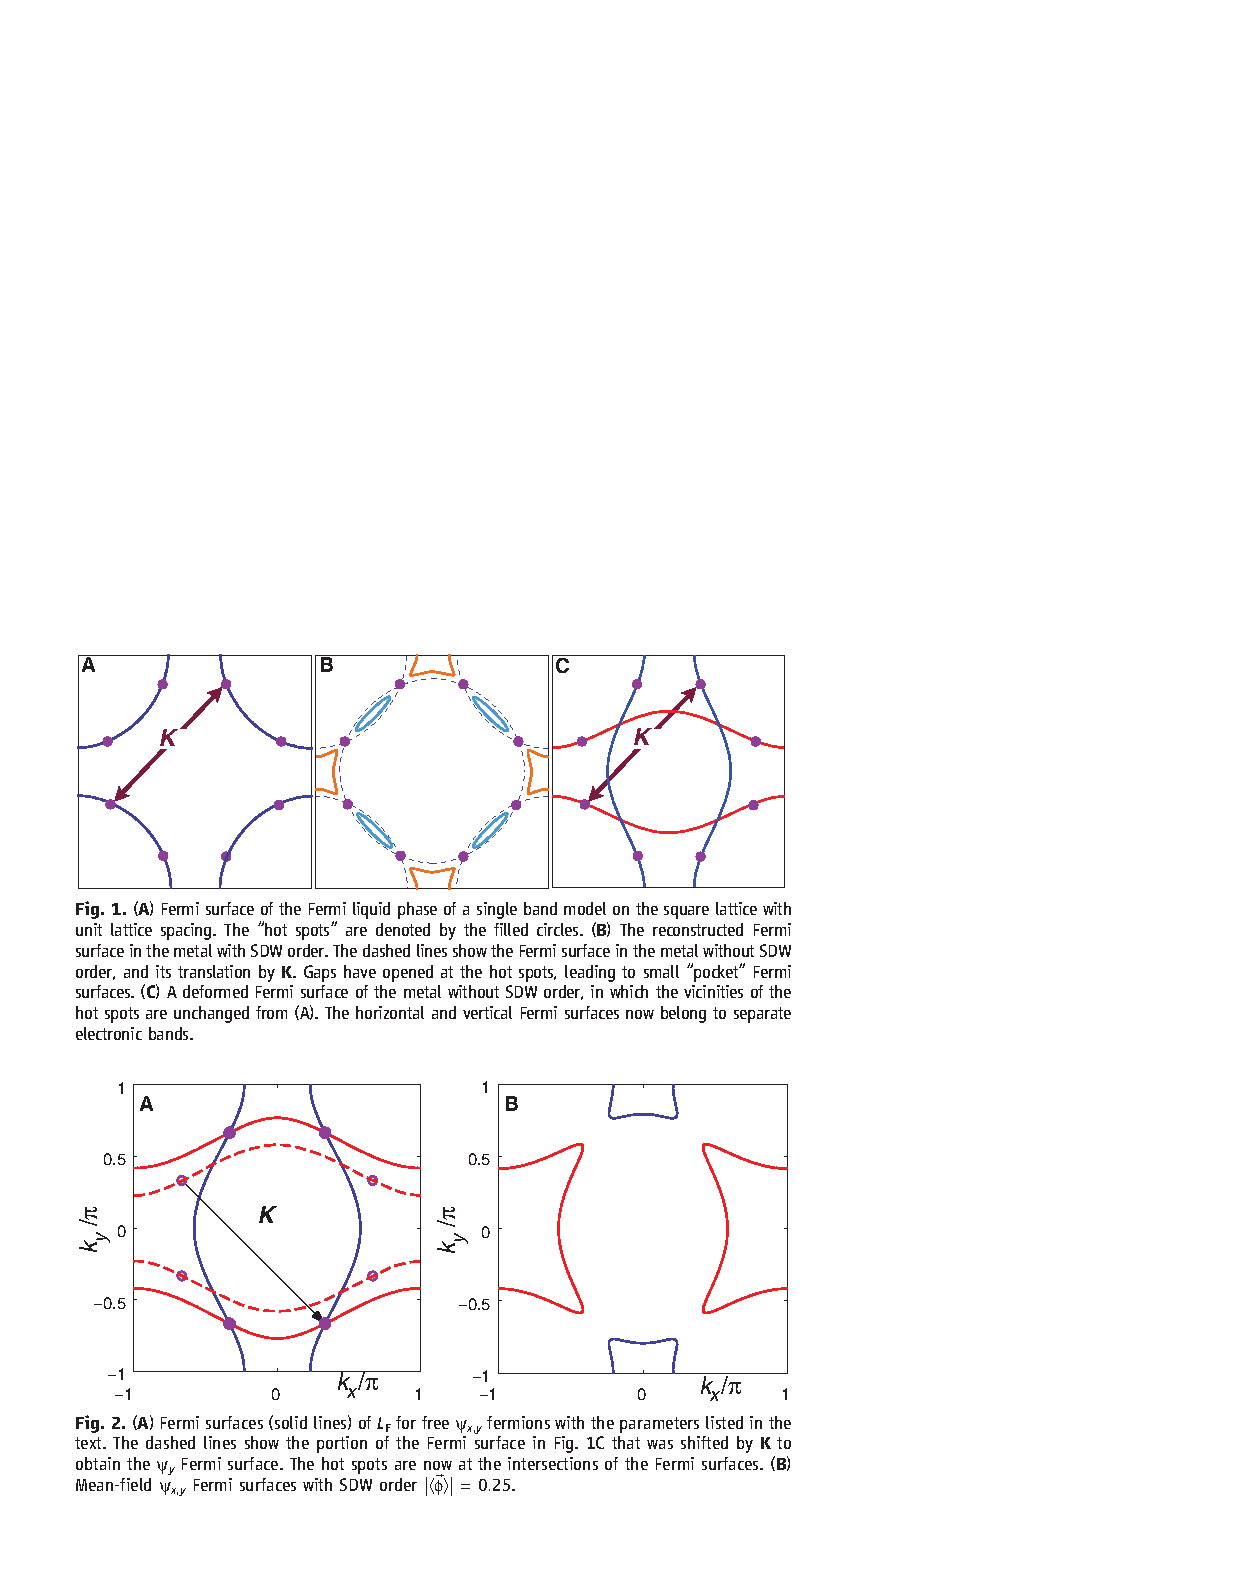
\includegraphics[width=\columnwidth]{berg2012}
	\end{center}
	\column{.4\textwidth}
	\begin{itemize}
		\item E Berg, M Metlitski and S Sachdev,\\ Science 2012.
		\item Use a two-band model to simulate SDW instability in cuprates.
		\item Two-band model removes sign problem.
	\end{itemize}
\end{columns}
\end{frame}

\begin{frame}
	\frametitle{Simulating effective models of spin liquids}
	\begin{columns}
		\column{.5\textwidth}
		\begin{center}
			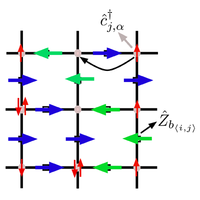
\includegraphics[width=4cm]{z2dsl}
		\end{center}
		\begin{itemize}
			\item F Assaad and T Grover, PRX 2016
			\item S Gazit, M Randeria and A Vishwanath, Nat Phys 2017
			\item Simulated $\mathbb Z_2$-Dirac spin liquid
		\end{itemize}
		\column{.5\textwidth}
		\begin{center}
			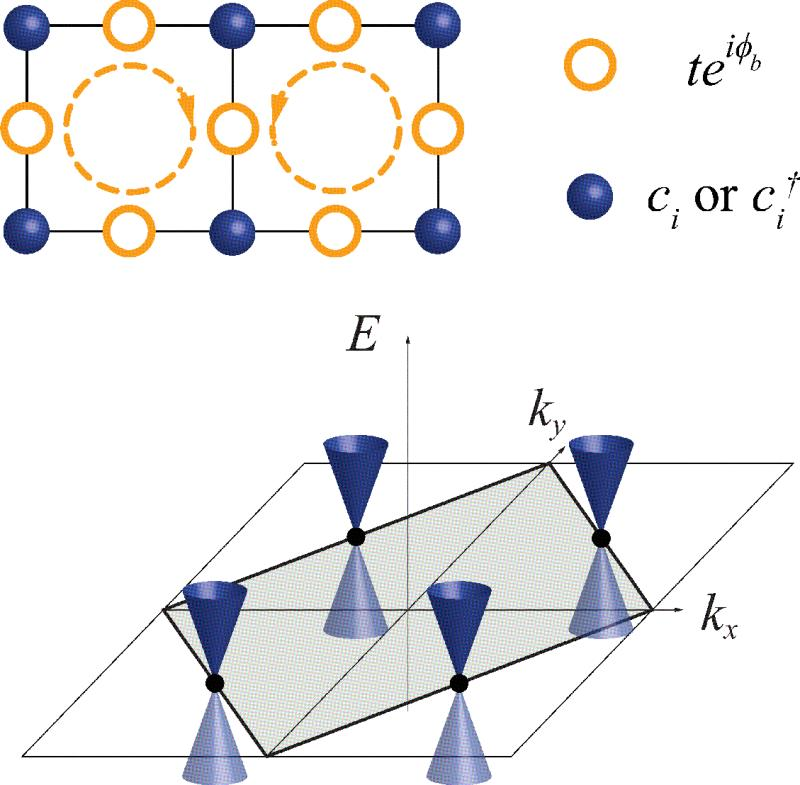
\includegraphics[width=4cm]{u1dsl}
		\end{center}
		\begin{itemize}
			\item Xiao Yan Xu, Yang Qi, Long Zhang, F Assaad, Cenke Xu, and Zi Yang Meng, PRX 2019
			\item Simulated U(1)-Dirac spin liquid.
		\end{itemize}
	\end{columns}
\end{frame}

\section{Model}

\begin{frame}
	\frametitle{The Model}
\begin{itemize}
\item Hamiltonian:
	\begin{align*}
	H_f &= -t\sum_{\langle i,j \rangle} (f^{\dagger}_{i,\alpha} \sigma^{z}_{b_{\langle i,j \rangle}}f_{j,\alpha} + h.c.) -\mu\sum_{i}f^{\dagger}_{i,\alpha}f_{i,\alpha}, \nonumber\\
	H_{z} &= -J \sum_{\langle i,j \rangle} S^{z}_{i} \sigma^{z}_{b_{\langle i,j \rangle}} S^{z}_{j} - h \sum_{i} S^{x}_{i}, \nonumber\\
	H_{g} &= -K \sum_{\square}\prod_{b\in\square} \sigma^{z}_{b} - g\sum_{b} \sigma^{x}_{b}.
\end{align*}
\item Physical fermion $c_{i\alpha} = f_{i\alpha}S_i^z$
\end{itemize}
\begin{center}
	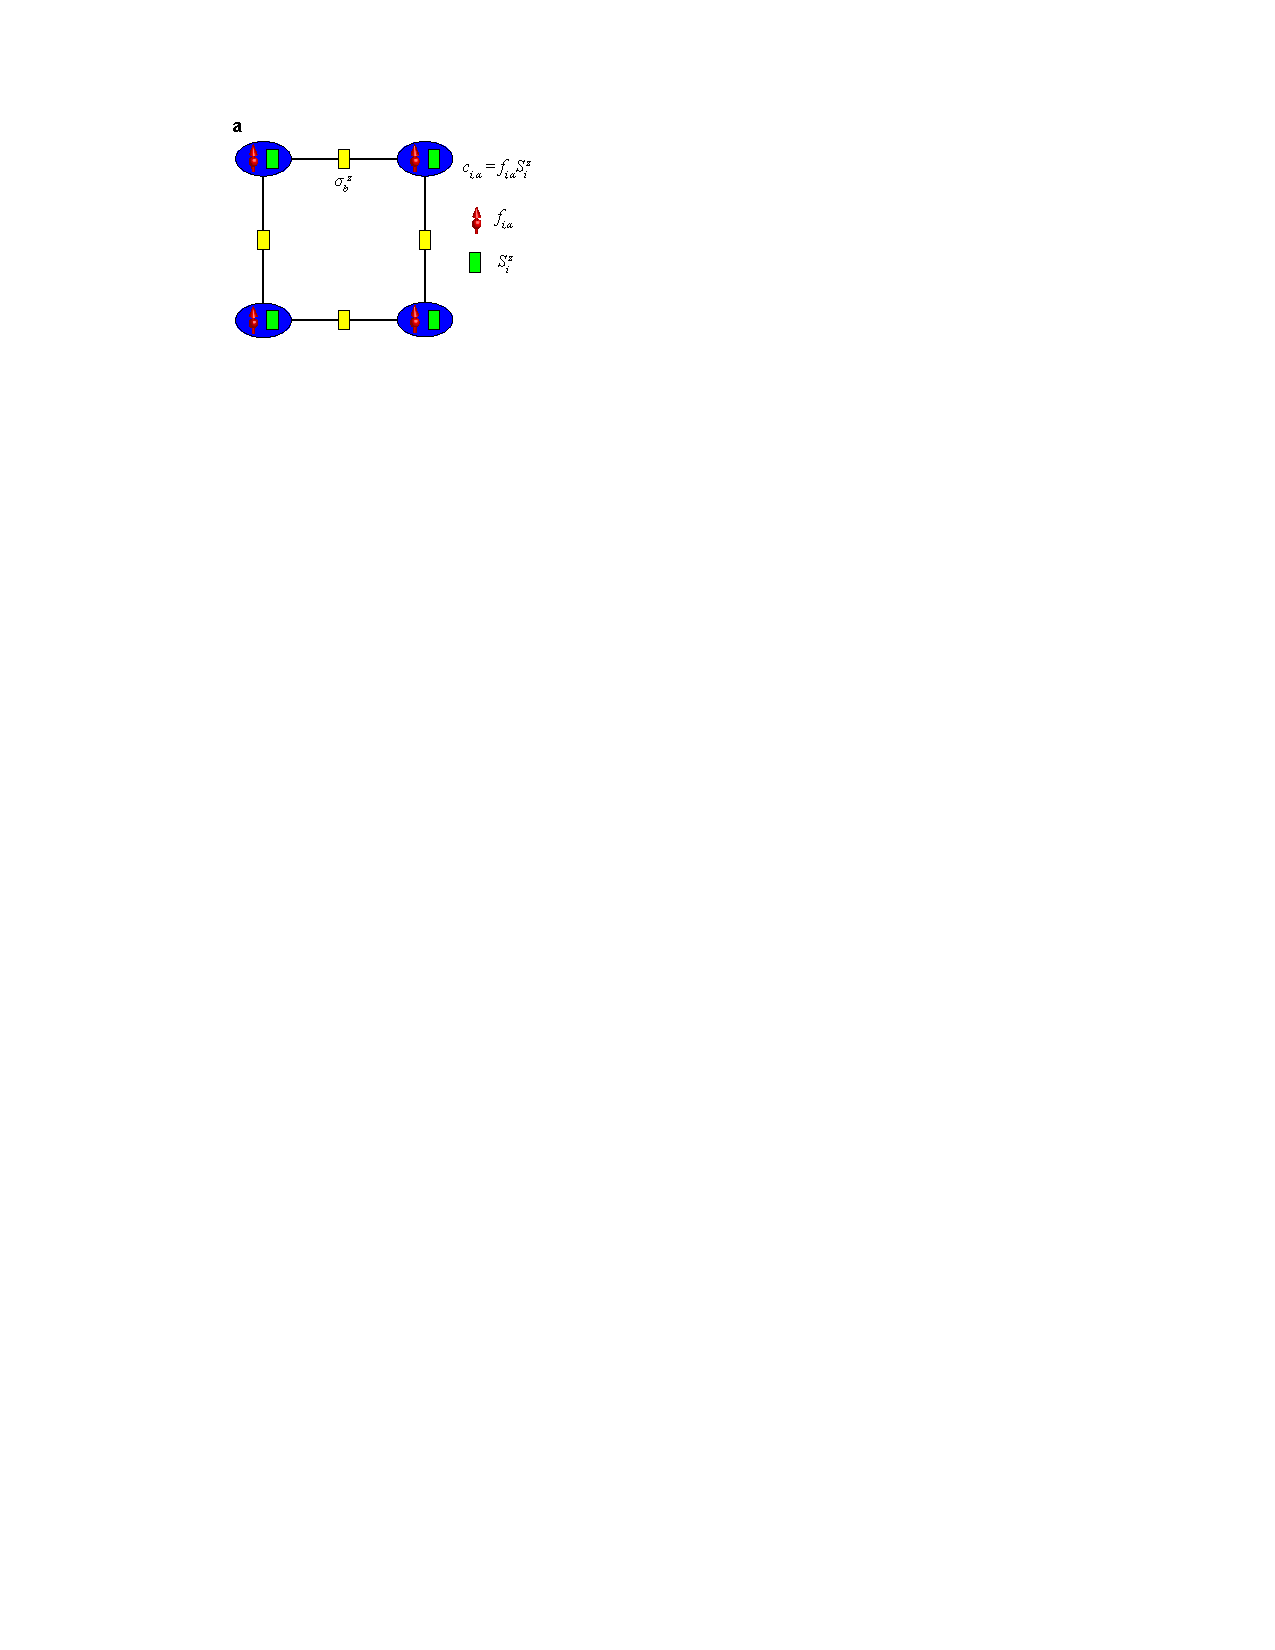
\includegraphics[width=4cm]{model_l}
\end{center}
\end{frame}

\begin{frame}
\frametitle{Symmetries -- I}
\begin{align*}
	H= &-t\sum_{\langle i,j \rangle} (f^{\dagger}_{i,\alpha} \sigma^{z}_{b_{\langle i,j \rangle}}f_{j,\alpha} + h.c.)
	-J \sum_{\langle i,j \rangle} S^{z}_{i} \sigma^{z}_{b_{\langle i,j \rangle}} S^{z}_{j} - h \sum_{i} S^{x}_{i}\\
&-K \sum_{\square}\prod_{b\in\square} \sigma^{z}_{b} - g\sum_{b} \sigma^{x}_{b}.
\end{align*}
\begin{enumerate}
\item $\mathbb Z_2$ gauge symmetry:
\[f_{i\alpha}\rightarrow\eta_if_{i\alpha},
\quad S_i^z\rightarrow\eta_iS_i^z,
\quad \sigma_{ij}\rightarrow
\eta_i\sigma_{ij}\eta_j.\]
\end{enumerate}
\begin{block}{Gauge constraint}
\begin{itemize}
\item Local projector $Q_i = (-)^{n_{i,f}}S^{x}_{i}\prod_{b\in +_i}\sigma^{x}_{b}$, w/ $n_{i,f}=\sum_{\alpha}f^{\dagger}_{i,\alpha}f_{i,\alpha}$.
\item $\hat Q_i=1$: Gauss Law.
\item $\hat Q_i\simeq1$ at low temperature: dynamically generated gauge-constraint.
\end{itemize}
\end{block}
\end{frame}

\begin{frame}
\frametitle{Symmetries -- II}
\begin{align*}
	H= &-t\sum_{\langle i,j \rangle} (f^{\dagger}_{i,\alpha} \sigma^{z}_{b_{\langle i,j \rangle}}f_{j,\alpha} + h.c.)
	-J \sum_{\langle i,j \rangle} S^{z}_{i} \sigma^{z}_{b_{\langle i,j \rangle}} S^{z}_{j} - h \sum_{i} S^{x}_{i}\\
&-K \sum_{\square}\prod_{b\in\square} \sigma^{z}_{b} - g\sum_{b} \sigma^{x}_{b}.
\end{align*}
\begin{enumerate}
	\addtocounter{enumi}{1}
\item $\mathbb Z_2$ \alert{global} symmetry:
$S_i^z\rightarrow -S_i^z$.
\item U(1) symmetry:
$f_{i\alpha}\rightarrow f_{i\alpha}e^{i\theta}$, $c_{i\alpha}\rightarrow c_{i\alpha}e^{i\theta}$.
$\Rightarrow$ Luttinger Theorem.
\end{enumerate}
\begin{block}{Ising symmetry is not really a global symmetry}
\begin{itemize}
\item Ising symmetry + fermion-parity symmetry $\in$ gauge symmetry:\\
$S_i^z\rightarrow-S_i^z,f_{i\alpha}\rightarrow-f_{i\alpha}$.
\item $\langle S_i^z\rangle\neq0$ is a \alert{Higgs} transition:
no\ bosonic local order parameter.
\end{itemize}
\end{block}
\end{frame}

\begin{frame}
\frametitle{Gauge symmetry and string operators}
\begin{itemize}
\item Gauge symmetry can never be broken.
\item Path integral / Monte Carlo sums over all gauge-equivalent configurations.
\item If $\hat O$ is not gauge invariant,
$\langle\hat O\rangle = 0$.
\item $\langle S_i^zS_j^z\rangle = 0$.
Need to use String operator $\langle S_i^z\sigma^z_{ii_1}\cdots\sigma^z_{i_nj}S_j^z\rangle$.
\item $\langle f_{i\alpha}f_{j\alpha}^\dagger\rangle=0$, $\langle c_{i\alpha}c_{j\alpha}^\dagger\rangle$ is Ok.
\end{itemize}

\begin{center}
	\begin{tikzpicture}
		\draw (0, 0)--(4, 0);
		\draw (0, 1)--(4, 1);
		\draw (0, 2)--(4, 2);
		\draw<1,3> (0, 3)--(4, 3);
		\draw (0, 4)--(4, 4);
		\draw (0, 0)--(0, 4);
		\draw (1, 0)--(1, 4);
		\draw (2, 0)--(2, 4);
		\draw<1,3> (3, 0)--(3, 4);
		\draw (4, 0)--(4, 4);
		\draw [thick,->,color=mbg] (0.9, 0.7)--(1.1, 1.3);
		\draw<1,3> [thick,->,color=mbg] (2.9, 2.7)--(3.1, 3.3);
		\draw<2> [thick,->,color=mbg] (3.1, 3.3)--(2.9, 2.7);
		\draw<2> [dashed] (2, 3)--(4, 3);
		\draw<2> (0, 3)--(2, 3);
		\draw<2> [dashed] (3, 2)--(3, 4);
		\draw<2> (3, 0)--(3, 2);
		\draw<3> [line width=2,blue] (1, 1)--(2, 1)--(2, 3)--(3, 3);
	\end{tikzpicture}
	\end{center}
\end{frame}

\section{Results}

\begin{frame}
\frametitle{Normal metal phase}
\begin{columns}
\column{.4\textwidth}
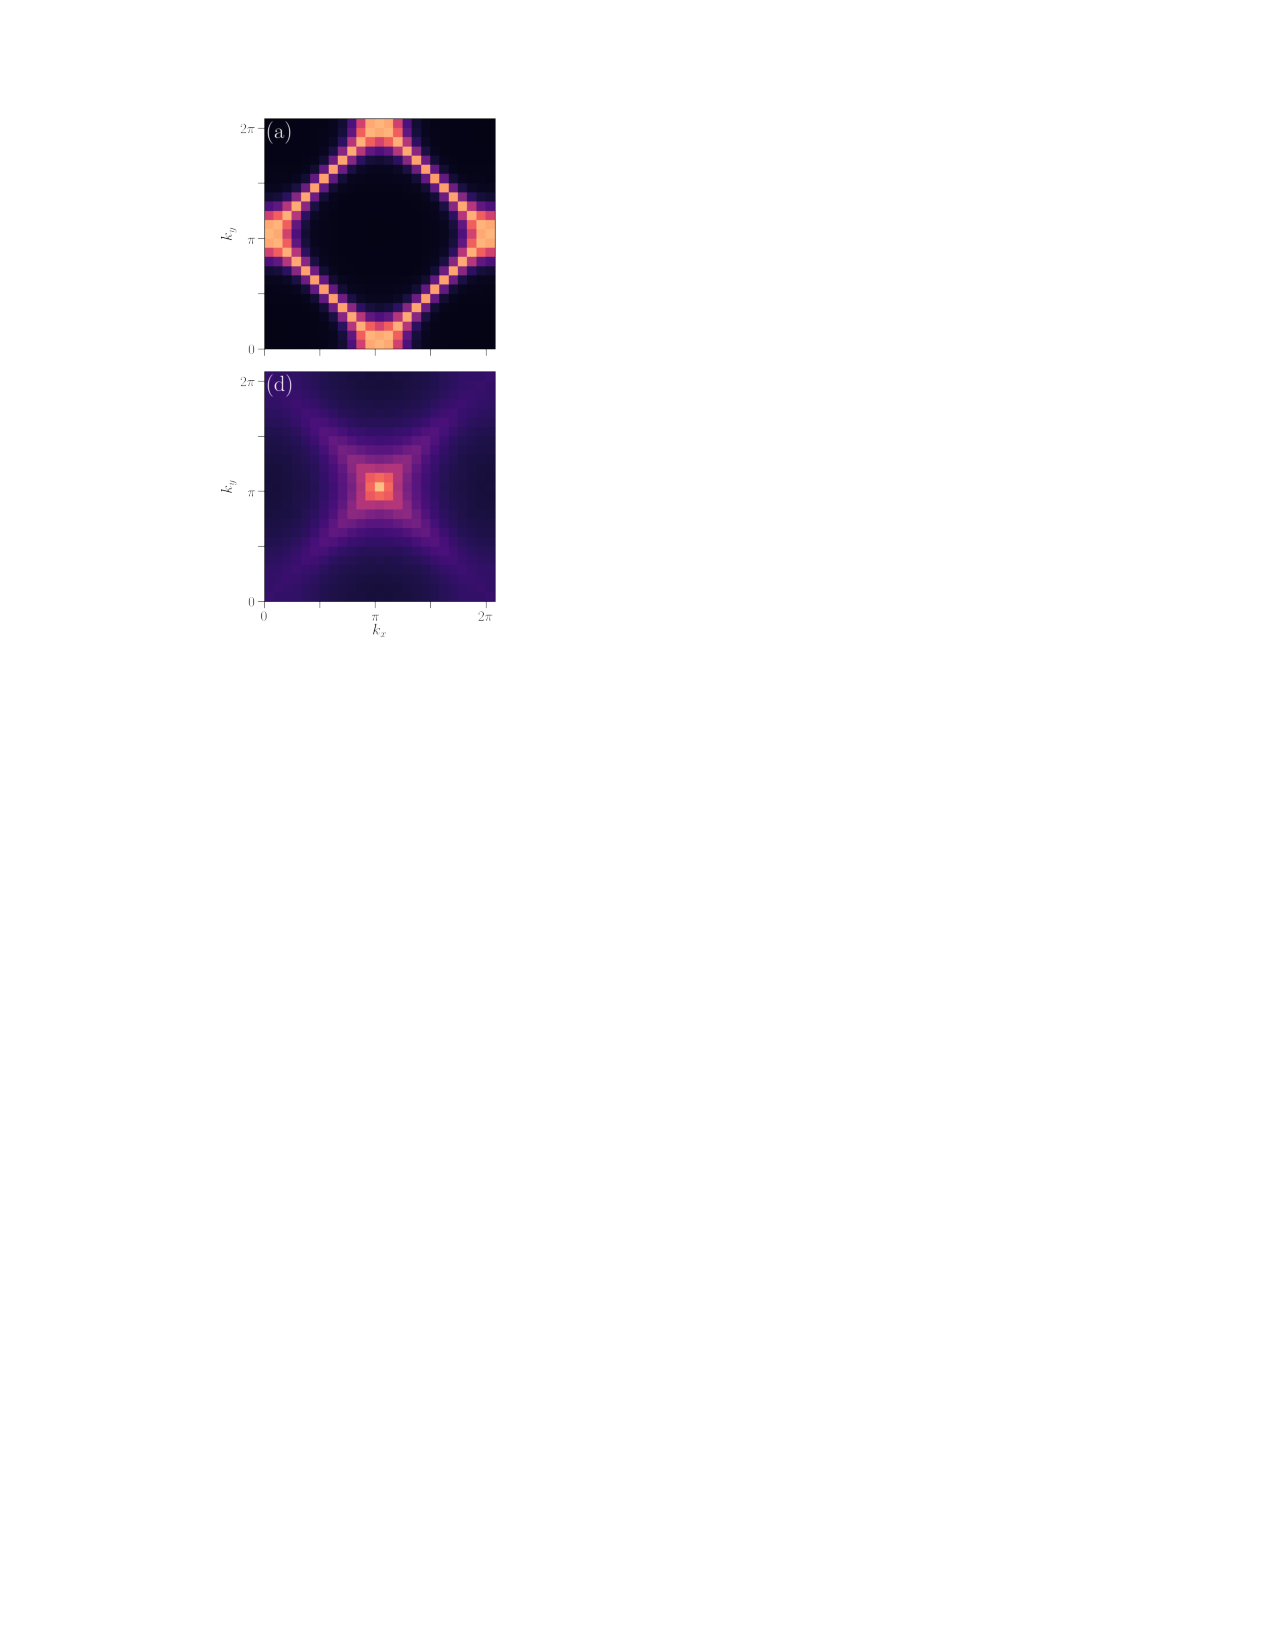
\includegraphics[width=\columnwidth]{nm}
\column{.6\textwidth}
\begin{itemize}
\item $h^z < h_c^z$: ``FM'' phase, ``$\langle S_i^z\rangle\neq0$''.
\item Higgs phase: $\mathbb Z_2$ gauge field is ``Higgs-ed''.
\item $c_{i\alpha} = S_i^zf_{i\alpha}\sim f_{i\alpha}$ forms a Fermi surface.
\item Susceptibility
$\chi_{ij}=\langle \vec s_i\cdot\vec s_j\rangle$,
$\vec s_i=c_{i\alpha}^\dagger\vec\sigma_{\alpha\beta}c_{i\beta}$ has a peak @ $(\pi,\pi)$.
\item A Landau Fermi liquid.
\end{itemize}
\end{columns}
\end{frame}

\begin{frame}
\frametitle{Orthogonal metal phase}
\begin{columns}
	\column{.4\textwidth}
	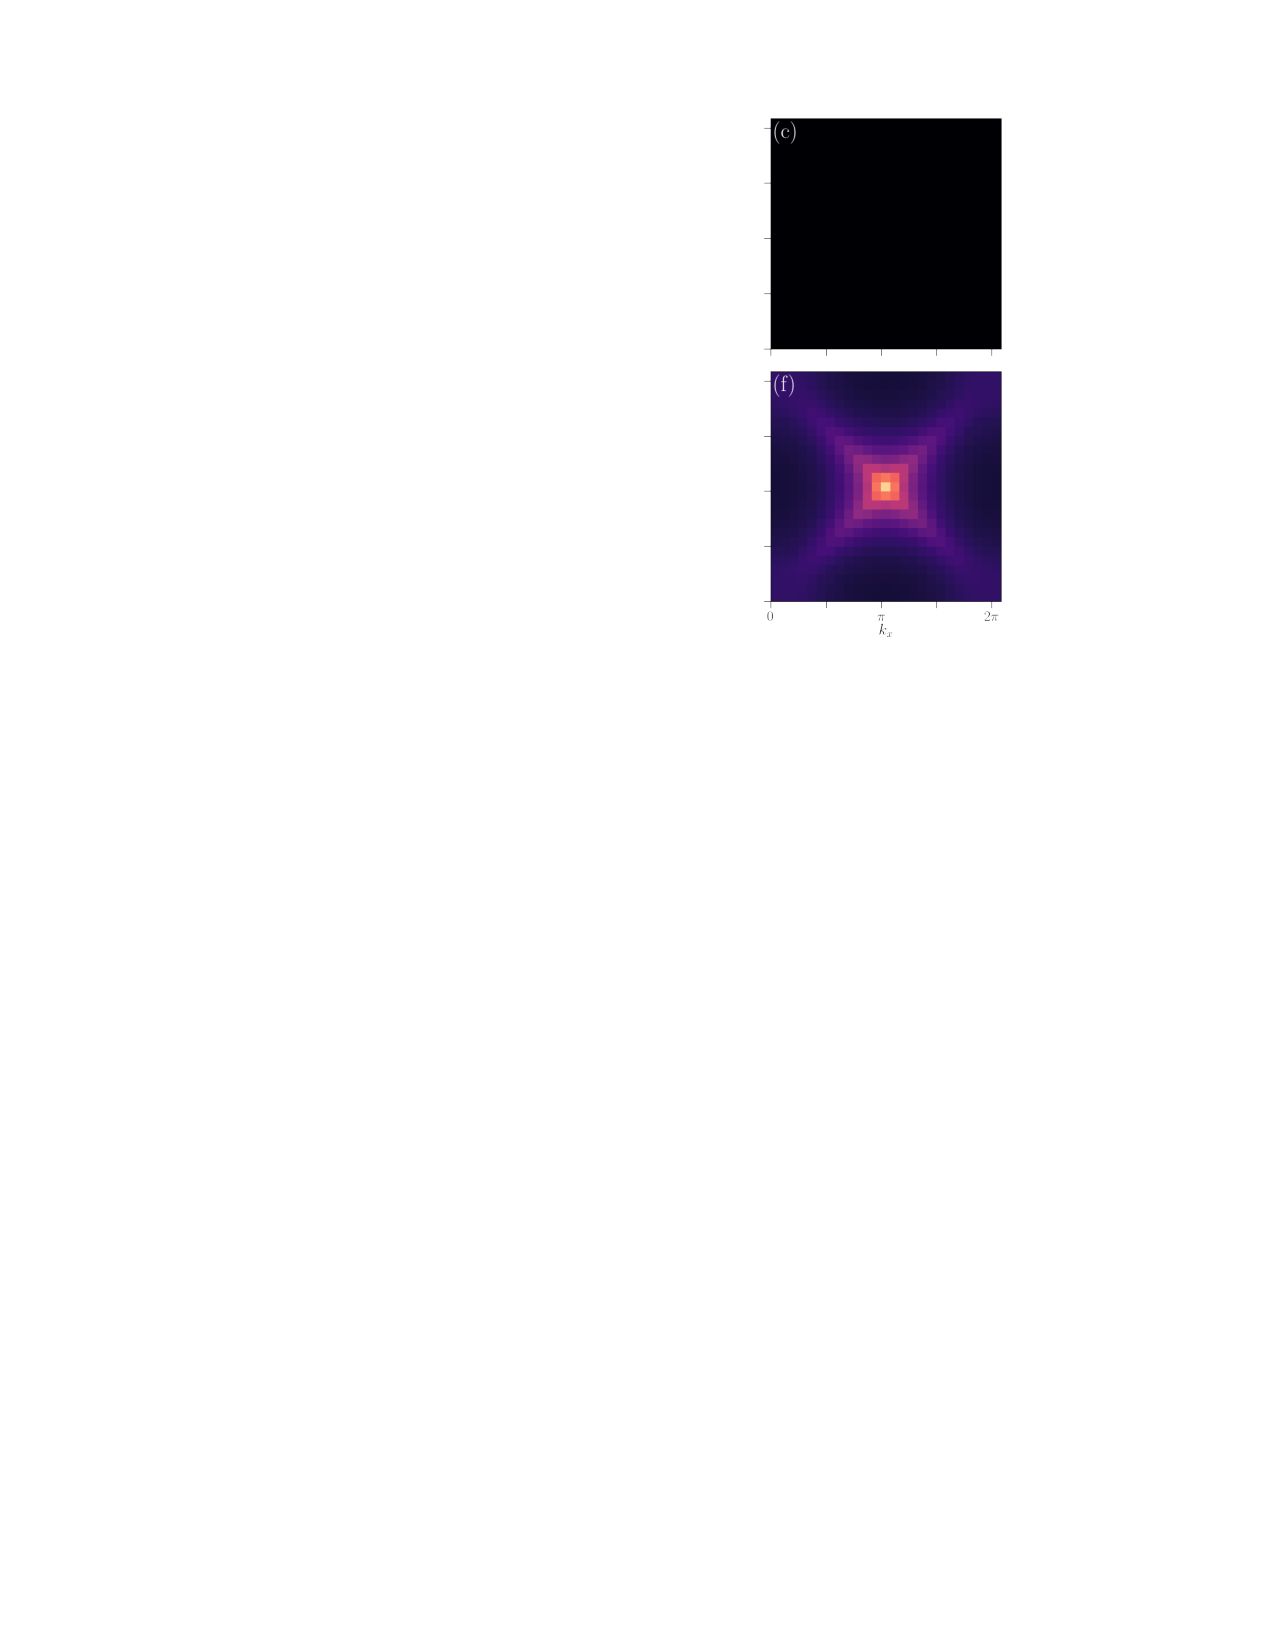
\includegraphics[width=.9\columnwidth]{om}
	\column{.6\textwidth}
	\begin{itemize}
	\item $h^z > h_c^z$: ``PM'' phase, ``$\langle S_i^z\rangle=0$''.
	\item $\mathbb Z_2$ gauge field is deconfined.
	\item Cannot find a $c$-fermion Fermi surface.
	\item Susceptibility still has a peak @ $(\pi,\pi)$: $\vec s_i= c_{i\alpha}^\dagger\vec\sigma_{\alpha\beta}c_{i\beta}
	= f_{i\alpha}^\dagger\vec\sigma_{\alpha\beta}f_{i\beta}$.
	\item A hidden $f$-fermion Fermi surface.
	\item A non-Fermi liquid: $\nu_e = A_f$ instead of $A_c$.
	\end{itemize}
\end{columns}
\end{frame}

\begin{frame}
\frametitle{Phase diagram}
\begin{itemize}
\item $c$-FS disappears.
\item Susceptibility peak remains $\Rightarrow$ a hidden $f$-FS.
\end{itemize}
\begin{center}
	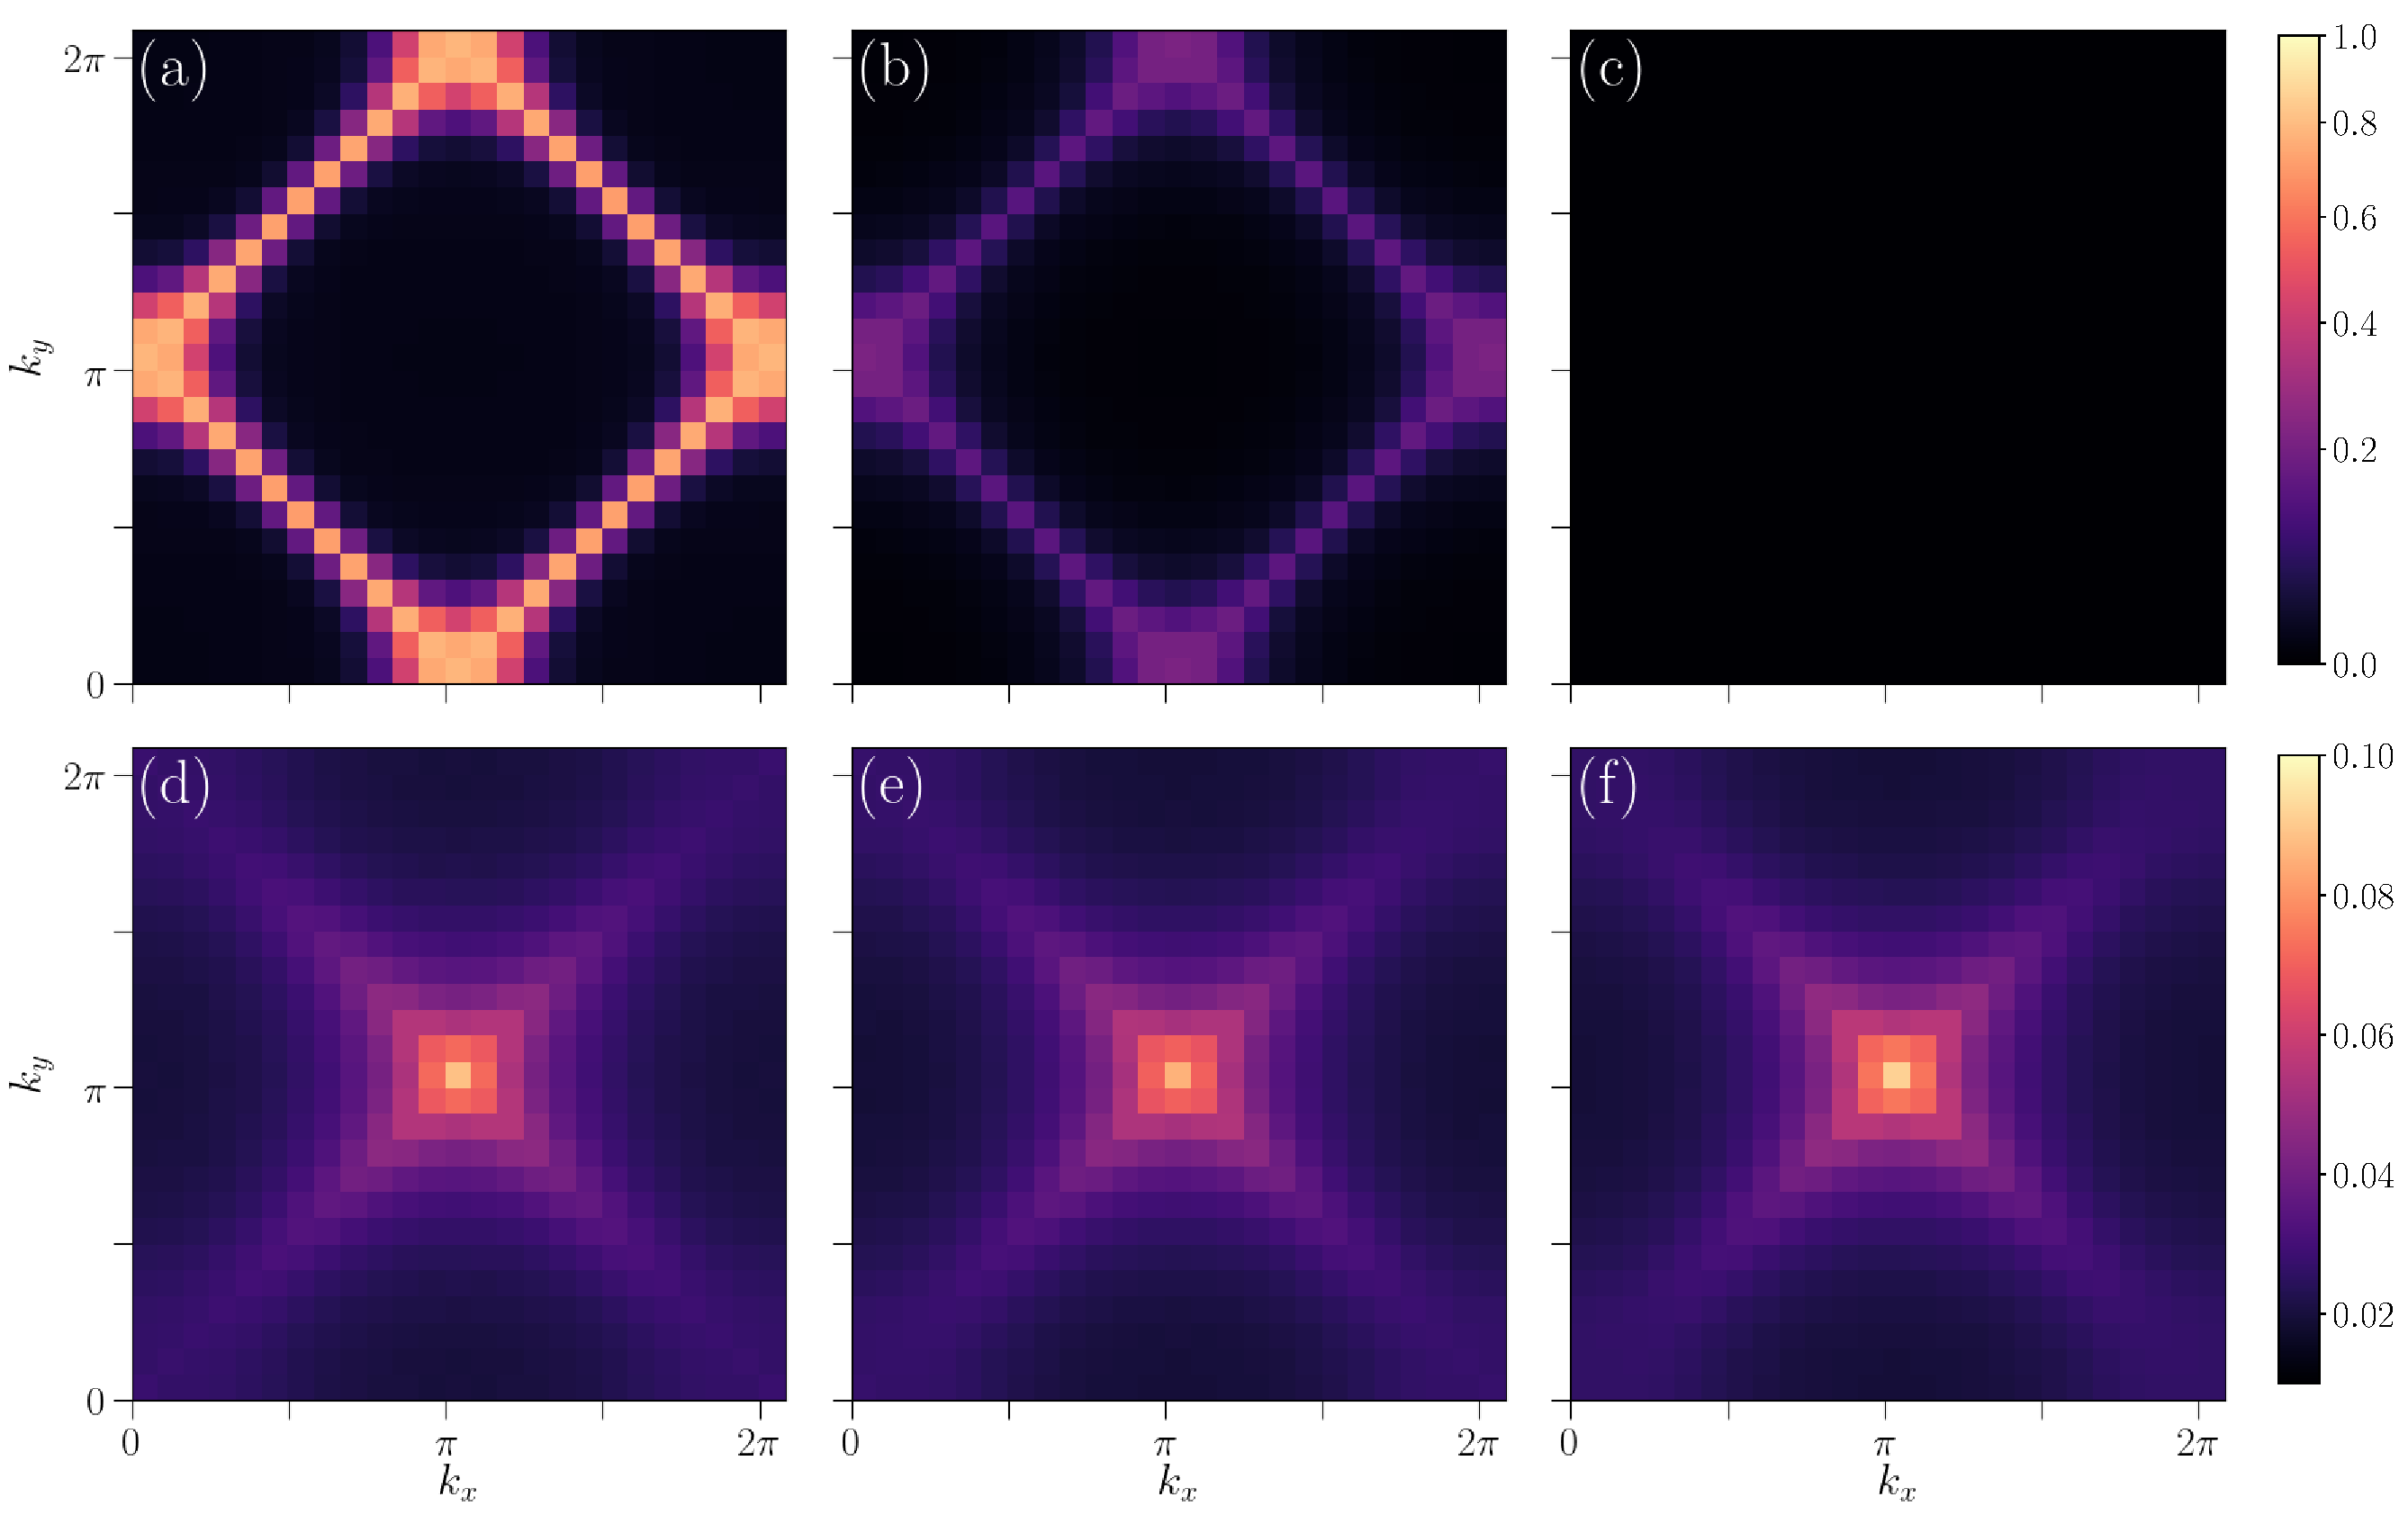
\includegraphics[width=\textwidth]{fig2}
\end{center}
\end{frame}

\begin{frame}
\frametitle{Phase diagram}
\begin{itemize}
\item $c$-FS disappears.
\item Susceptibility peak remains $\Rightarrow$ a hidden $f$-FS.
\end{itemize}
\begin{center}
	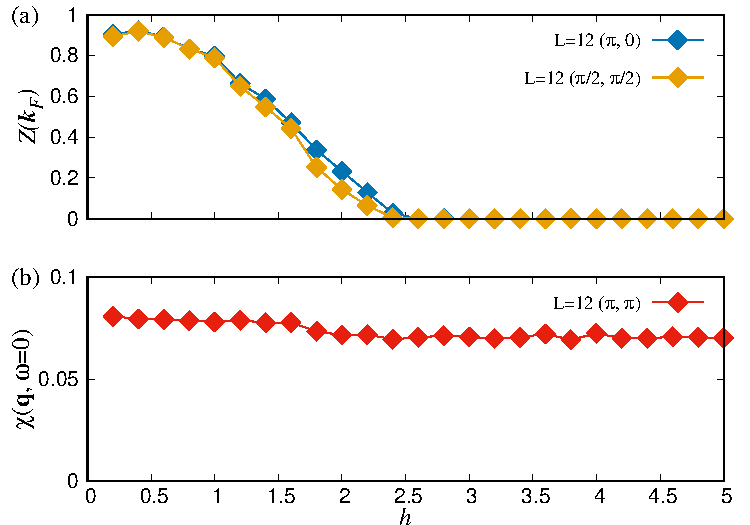
\includegraphics[width=.8\textwidth]{fig4}
\end{center}
\end{frame}

\begin{frame}
\frametitle{Away from half-filling}
\begin{center}
	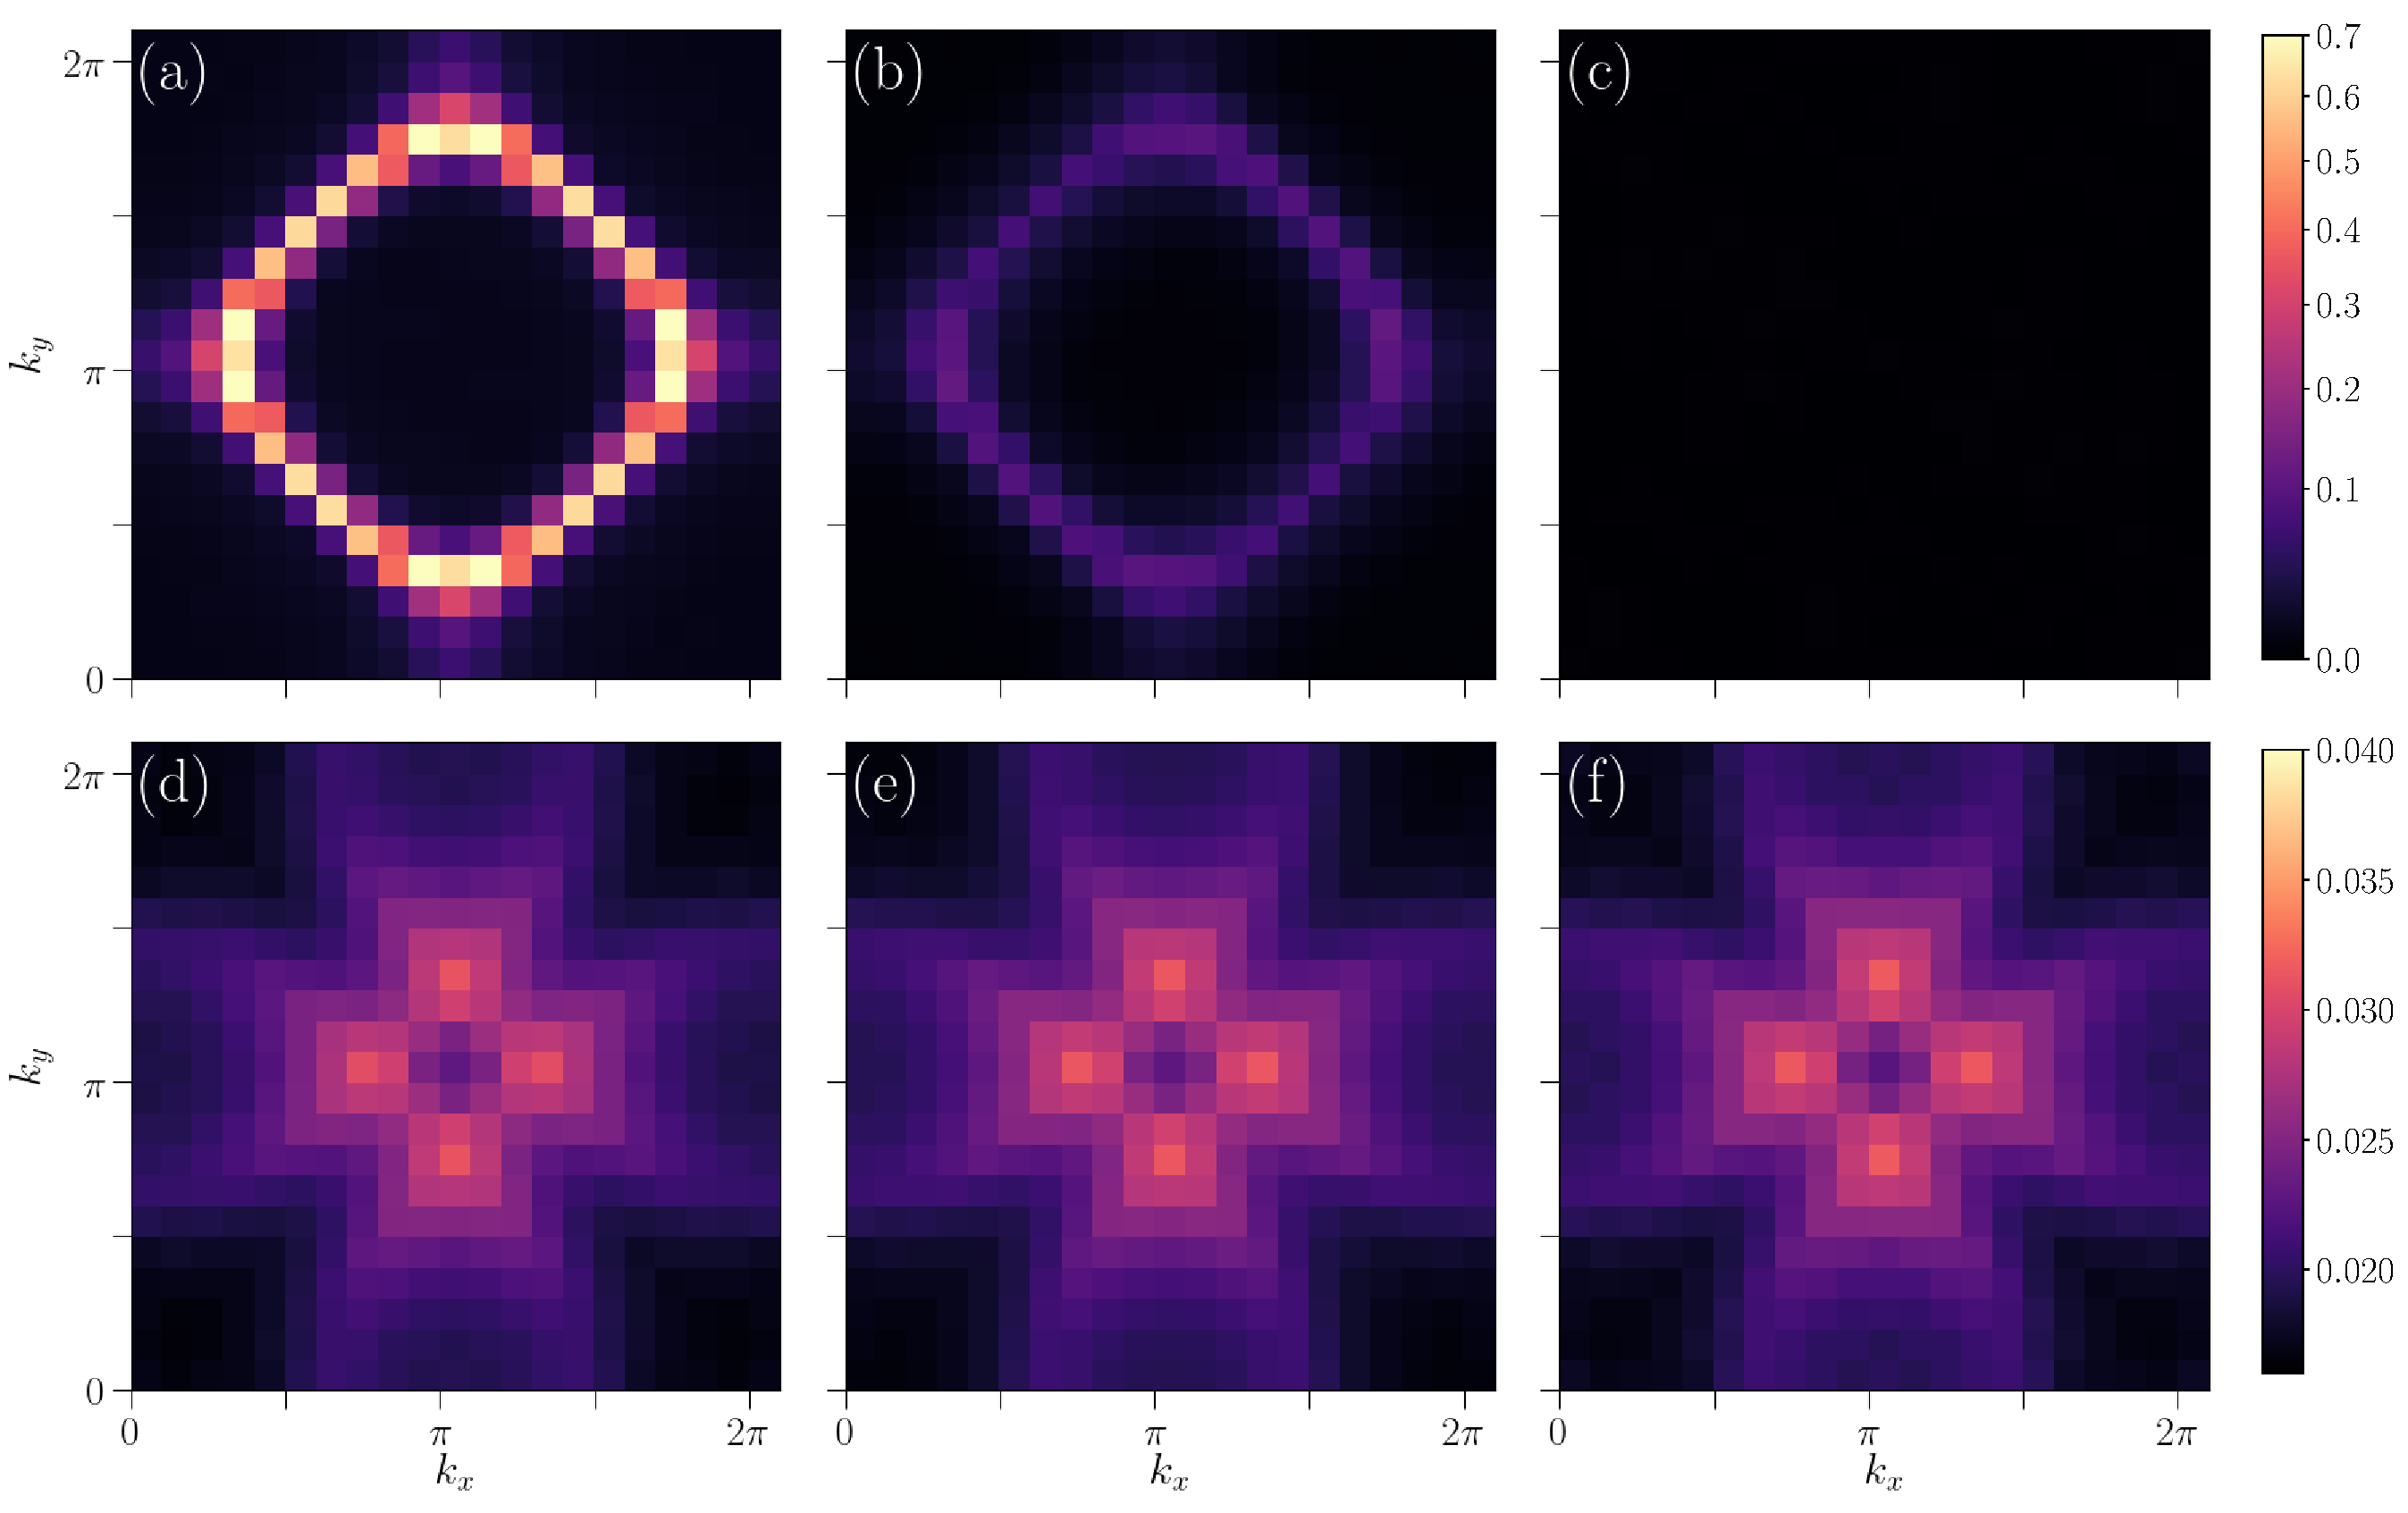
\includegraphics[width=\textwidth]{figS1}
\end{center}
\end{frame}

\begin{frame}
\frametitle{The Higgs transition}
\begin{center}
	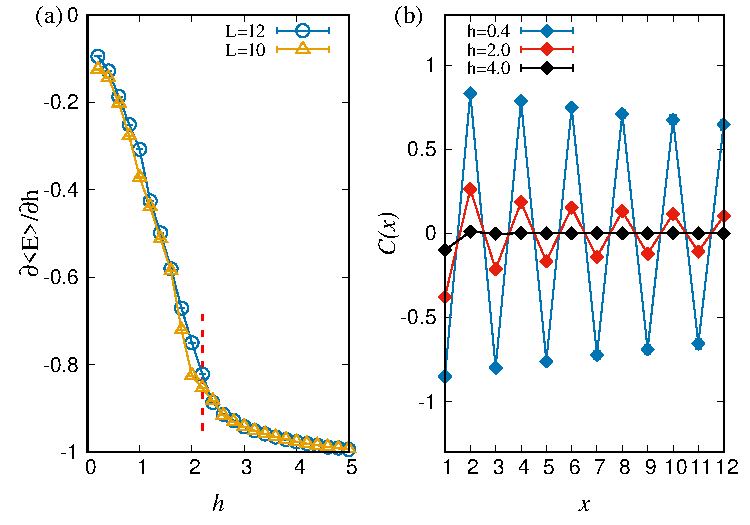
\includegraphics[height=5cm]{fig3}
\end{center}
\begin{itemize}
	\item Appears to be continuous.
	\item Hidden order: $\langle S_i^z\sigma^z\cdots\sigma^zS_j^z\rangle$.
	\item Not 3D Ising:
	$\mathcal L = (\partial_\mu\phi)^2-r\phi^2+u\phi^4+\phi^2\psi^\dagger\sigma^z\psi+\cdots$.
	\item Weak first-order? Sachdev and Morinari [PRB, 66, 235117 (2017)].
\end{itemize}
\end{frame}

\section{Conclusion}
\begin{frame}{Conclusion and Outlook}
\begin{center}
	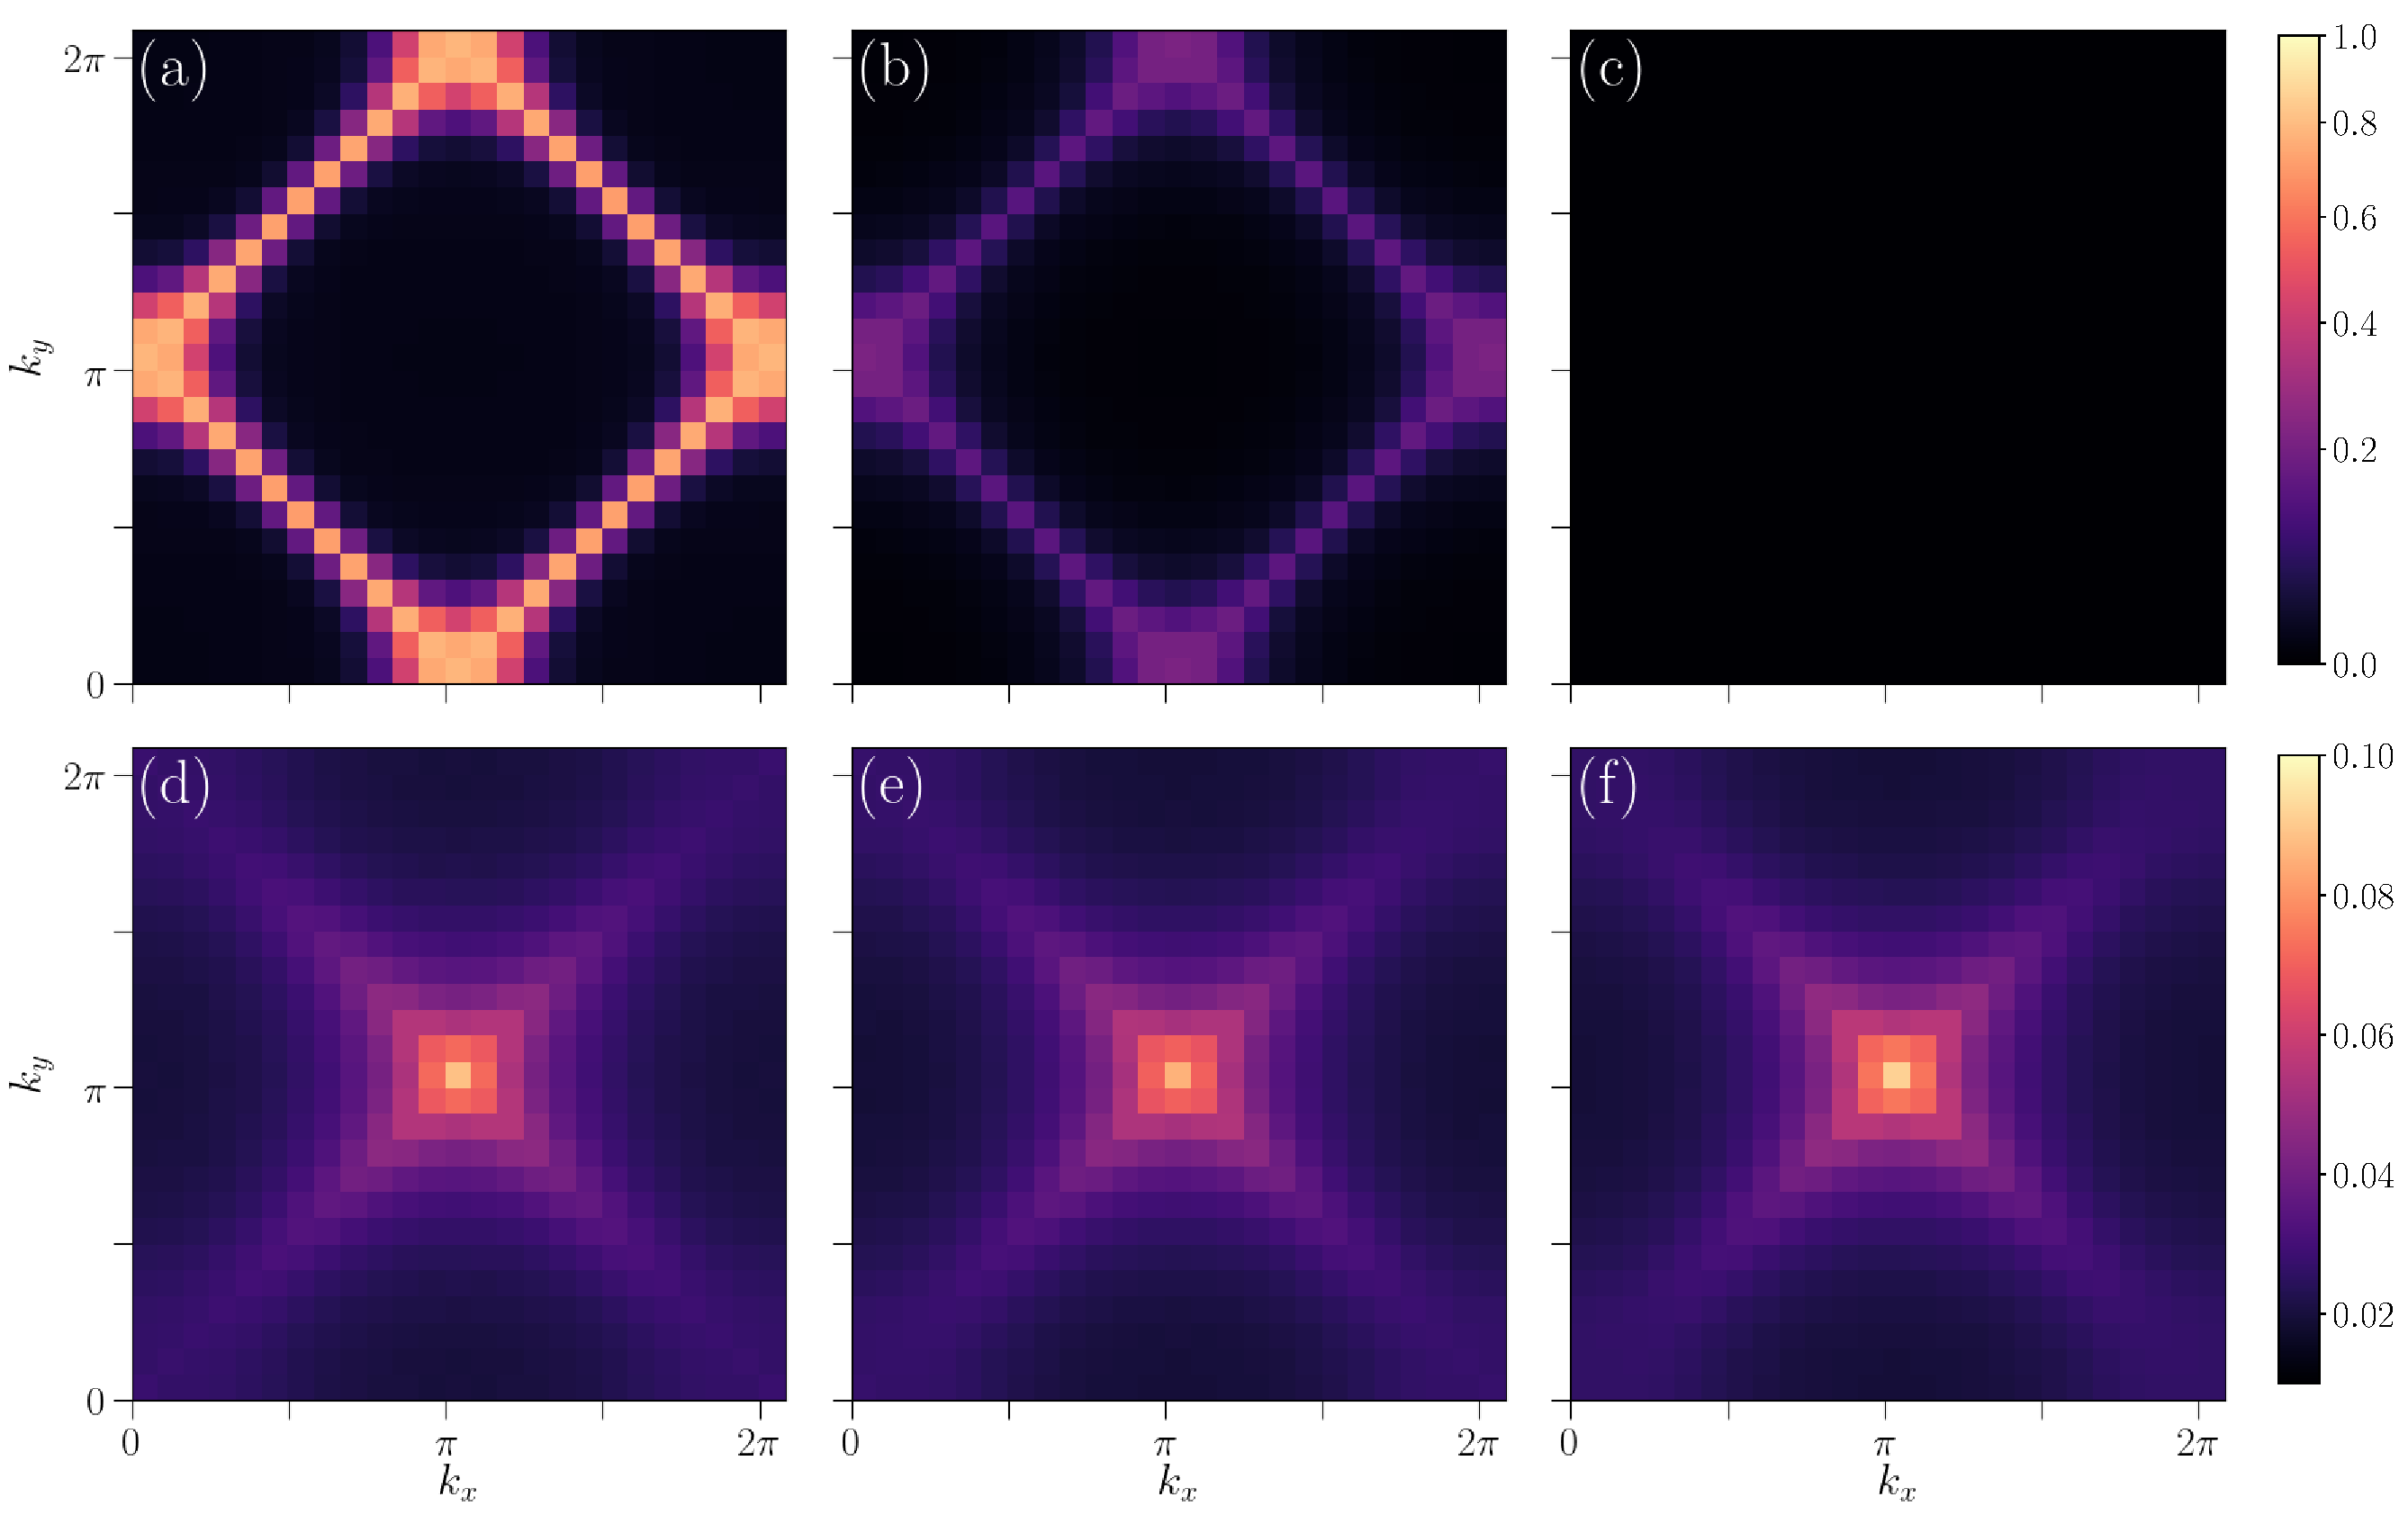
\includegraphics[width=.6\textwidth]{fig2}
\end{center}
\begin{itemize}
\item Metals' awkwark cousin is found.
\item Demonstrated an OM phase using MC simulation.
\item Higgs transition: appears to be continuous.
\item Spin liquid w/ spinon FS: U(1) spin liquid?
\item Nature of the phase transition?
\end{itemize}
\end{frame}
\end{document}
